\documentclass[conference]{IEEEtran}

\usepackage{amsmath,amssymb}
\usepackage{graphicx}
\usepackage{cite}
\usepackage{booktabs}
\usepackage{array}
\usepackage{tabularx}
\usepackage{multirow}
\usepackage{url}
\usepackage[hidelinks]{hyperref}
\usepackage{tikz}
\usetikzlibrary{arrows.meta,positioning,shapes.geometric,fit}

\newcolumntype{Y}{>{\raggedright\arraybackslash}X}
\newcommand{\pending}{\textit{Not yet measured}}

\tikzset{
  flow/.style={draw,rounded corners=2pt,align=center,minimum height=7mm,
    inner sep=3pt,font=\scriptsize},
  source/.style={flow,fill=blue!8},
  storage/.style={flow,fill=orange!12},
  process/.style={flow,fill=green!10},
  decision/.style={flow,fill=red!9},
  output/.style={flow,fill=violet!10},
  arrow/.style={-{Latex[length=2mm]},thick}
}

\title{An Exploratory District-Level Extreme-Precipitation and Response-Priority Prototype for Andhra Pradesh and Telangana}

% Center a second row of authors in the IEEE conference author block.
\makeatletter
\newcommand{\linebreakand}{%
  \end{@IEEEauthorhalign}%
  \hfill\mbox{}\par
  \mbox{}\hfill\begin{@IEEEauthorhalign}%
}
\makeatother

\author{
\IEEEauthorblockN{Balla Tenisha Akhila}
\IEEEauthorblockA{
School of Computing\\
Amrita Vishwa Vidyapeetham\\
Clappana, P.O. Kerala\\
tenishaakhilaballa@gmail.com}
\and
\IEEEauthorblockN{Bhupati Jeevita}
\IEEEauthorblockA{
School of Computing\\
Amrita Vishwa Vidyapeetham\\
Clappana, P.O. Kerala\\
bhupati.jeevita@gmail.com}
\and
\IEEEauthorblockN{Nidamanuru Uthakarsh Sai}
\IEEEauthorblockA{
School of Computing\\
Amrita Vishwa Vidyapeetham\\
Clappana, P.O. Kerala\\
nidamanuruuthkarsh@gmail.com}
\linebreakand
\IEEEauthorblockN{Meesala Jagapathi Naidu}
\IEEEauthorblockA{
School of Computing\\
Amrita Vishwa Vidyapeetham\\
Clappana, P.O. Kerala\\
jagapathinaidu07122006@gmail.com}
\and
\IEEEauthorblockN{Surapureddy Akhil Reddy}
\IEEEauthorblockA{
School of Computing\\
Amrita Vishwa Vidyapeetham\\
Clappana, P.O. Kerala\\
akhilreddy.surapureddy@gmail.com}
}

\begin{document}
\maketitle

\begin{abstract}
This paper reports an exploratory district-level extreme-precipitation and
response-priority prototype for Andhra Pradesh and Telangana, and separates
completed pilot evidence from the newer RADAR workflow that remains to be
evaluated. The completed legacy pilot expands two mapped subdivision-level monthly
rainfall series across 23 Census-2011 districts, yielding 31,740 district-month
rows; it does not contain 23 independent district weather histories. A
chronological 2006--2015 test evaluation of a next-month extreme-precipitation
label reports average precision (PR-AUC) of 0.1287 for a gradient-boosted model
and 0.1111 for its historical-count heuristic. However, the label climatology was
estimated over the full 1901--2015 record, including test years, so this result
is exploratory and is not a leakage-free estimate of prospective performance.
The prototype also computes a transparent composite response-priority score
from hazard, exposure, healthcare, mobility, and housing proxies. Its
2015 ranking comparison is descriptive only: hazard scores are tied within
subdivisions, making top-five overlap dependent on tie handling and the reported
rank-correlation p-value unsuitable as confirmatory evidence. The newer
gridded, calibrated, conformal, and allocation pipeline is a research design;
its event-replay and uncertainty-aware allocation outcomes are not reported as
completed experiments here. These limitations define the work still required
before claims of district-level forecasting or operational benefit are
justified.
\end{abstract}

\begin{IEEEkeywords}
Big Data Analytics, disaster response, Apache Spark, Hadoop HDFS,
multi-source data integration, Random Forest, risk prediction, resource
prioritization
\end{IEEEkeywords}

\section{Introduction}

\subsection{Background}
Disaster management is a data-intensive decision problem. Environmental
observations describe the intensity and evolution of a hazard; population data
represent the people exposed; hospitals and shelters describe response
capacity; roads affect reachability; and historical records reveal recurring
hazards and severity patterns. The Sendai Framework emphasizes that disaster
risk must be understood through hazard characteristics, exposure,
vulnerability, and capacity rather than through a single variable
\cite{sendai}. Consequently, rainfall or a predicted hazard label alone cannot
describe the operational urgency of a district with dense population, limited
healthcare, and weak transport connectivity.

These data are heterogeneous in schema, time scale, geographic resolution, and
quality. They may also be maintained by different agencies and grow as new
observations and event records are collected. Joint analysis is therefore both
an integration problem and a distributed data-processing problem. HDFS and
Spark provide an architecture in which raw data, intermediate products, feature
engineering, and machine-learning stages can share a common distributed
pipeline rather than depend on disconnected single-machine scripts.

\subsection{Disaster Response Prioritization Problem}
Disaster prediction and disaster response prioritization address different
questions. Prediction asks whether an event is likely and when it may occur.
Prioritization asks: given several affected or vulnerable districts, where
should limited resources be deployed first? Emergency authorities must make
this decision while rescue personnel, transport, medical assistance, shelter
space, and relief materials are constrained. Research in emergency-response AI
similarly distinguishes incident prediction and detection from resource
allocation and dispatch \cite{mukhopadhyay}. A risk estimate is therefore
necessary but insufficient for an immediate field priority.

\subsection{Motivation}
The early period after a severe event is commonly described operationally as a
``golden hour,'' because delays in recognizing the most urgent locations can
affect rescue, evacuation, medical treatment, and relief distribution. The
phrase is used here as a decision-timeliness motivation rather than as a fixed
clinical deadline. When weather, population, hospitals, roads, and event
history remain in separate silos, analysts must manually reconcile conflicting
signals before a district can be compared with its peers. A unified score does
not remove uncertainty, but it can make the evidence used for triage explicit
and reproducible.

\subsection{Problem Statement}
The research problem is to develop a distributed analytics framework that
integrates heterogeneous disaster-related data and produces a district-level
response-priority ranking by combining predicted hazard risk with population
exposure and infrastructure-accessibility conditions.

\subsection{Research Objectives}
The objectives are to: (1) design an HDFS--Spark framework for multi-source
disaster analytics; (2) integrate weather, population, hospital, road, and
historical disaster data; (3) construct district-level vulnerability and
accessibility indicators; (4) train a Spark MLlib Random Forest model for risk
classification; (5) formulate DDRPS; (6) rank districts by response urgency;
and (7) provide a dashboard for priority, risk, and resource interpretation.

\subsection{Contributions}
The proposed work contributes: (1) a distributed multi-source disaster
analytics architecture; (2) district-level fusion of environmental,
demographic, healthcare, transportation, and historical information; (3) a
feature-engineering scheme for exposure, event frequency, severity, and access
deficits; (4) an MLlib Random Forest risk component; (5) DDRPS, which converts
risk and operational conditions into a comparable ranking; and (6) a
dashboard-oriented decision-support layer. The distinction between
\emph{predicted risk} and \emph{response priority} is maintained throughout.

\subsection{Paper Organization}
Section II positions the work within disaster analytics and allocation
literature. Sections III--VIII present the architecture, data processing,
feature engineering, risk model, DDRPS, and big-data pipeline. Sections IX and
X define the experimental protocol and report the current evidence boundary.
Sections XI--XIV discuss implications, limitations, future work, and
conclusions.

\section{Related Work}

\subsection{Social Media and Data Analytics in Disaster Response}
Large-scale disaster analytics has frequently used social media for event
detection, information extraction, communication, and situational awareness.
Imran \emph{et al.} survey computational processing of emergency messages
\cite{imran}, while Karimiziarani reviews collection, preprocessing, mining,
and ethical issues in disaster-oriented social media analytics
\cite{karimiziarani}. Recent work studies actual emergency-management usage
patterns \cite{purohit}, earthquake-response information flows
\cite{kopanov}, and multi-label disaster-text classification
\cite{crisissense}. These approaches can improve awareness of what is
happening, but their primary output is usually extracted information or event
classification rather than a district-wise fusion of hazard, exposure, and
infrastructure for first-stage response ranking.

\subsection{Artificial Intelligence for Emergency Response}
AI-based emergency-response research covers incident prediction, detection,
allocation, and dispatch \cite{mukhopadhyay}. This breadth is important because
a high-quality prediction does not itself determine an operational allocation.
The proposed framework uses machine learning only for district risk estimation;
the final priority remains a transparent multi-indicator decision layer.

\subsection{Resource Allocation and Optimization}
Operations-research models have long addressed scarce-resource decisions in
disaster operations \cite{altay}. Zhang \emph{et al.} combine demand
prediction with stochastic optimization for proactive resource requests
\cite{zhang}. Xu \emph{et al.} formulate multi-cycle rescue allocation under
multiple objectives and constraints \cite{xu}. Such models can represent
complex operational details, but they require demand, capacity, objective, and
constraint specifications that may not be available during initial triage.
DDRPS is positioned before detailed routing or allocation: it identifies which
districts should enter those downstream processes first.

\subsection{Infrastructure- and Vulnerability-Aware Response}
Emergency planning increasingly considers evacuation, facilities, casualty
transport, search and rescue, and relief distribution together
\cite{pu}. Infrastructure and demographic context affect both the consequences
of a hazard and the feasibility of response. The present design operationalizes
that observation through population exposure, healthcare access deficit, road
access deficit, and a shelter proxy at one geographic unit.

\subsection{Research Gap}
Four gaps motivate the framework. First, the \emph{focus gap}: much predictive
work asks ``if/when,'' while authorities also require ``where first.'' Second,
the \emph{integration gap}: environmental, population, healthcare,
transportation, and historical sources are often studied separately. Third,
the \emph{scalability gap}: many decision prototypes do not explicitly place
data cleaning, joins, and learning in a distributed pipeline. Fourth, the
\emph{decision-support gap}: model outputs may not be converted into a single,
interpretable operational priority. The proposed framework bridges predictive
disaster analytics and actionable response prioritization without claiming to
replace detailed allocation optimization or human command decisions.

\section{Proposed System Architecture}

The overall architecture is shown in Fig.~\ref{fig:architecture}. Five source
families feed distributed storage. Spark performs cleaning, district-level
fusion, and feature construction. MLlib predicts risk, DDRPS combines risk with
exposure and access deficits, and a dashboard presents the resulting ranking.

\begin{figure*}[t]
\centering
\resizebox{0.98\textwidth}{!}{%
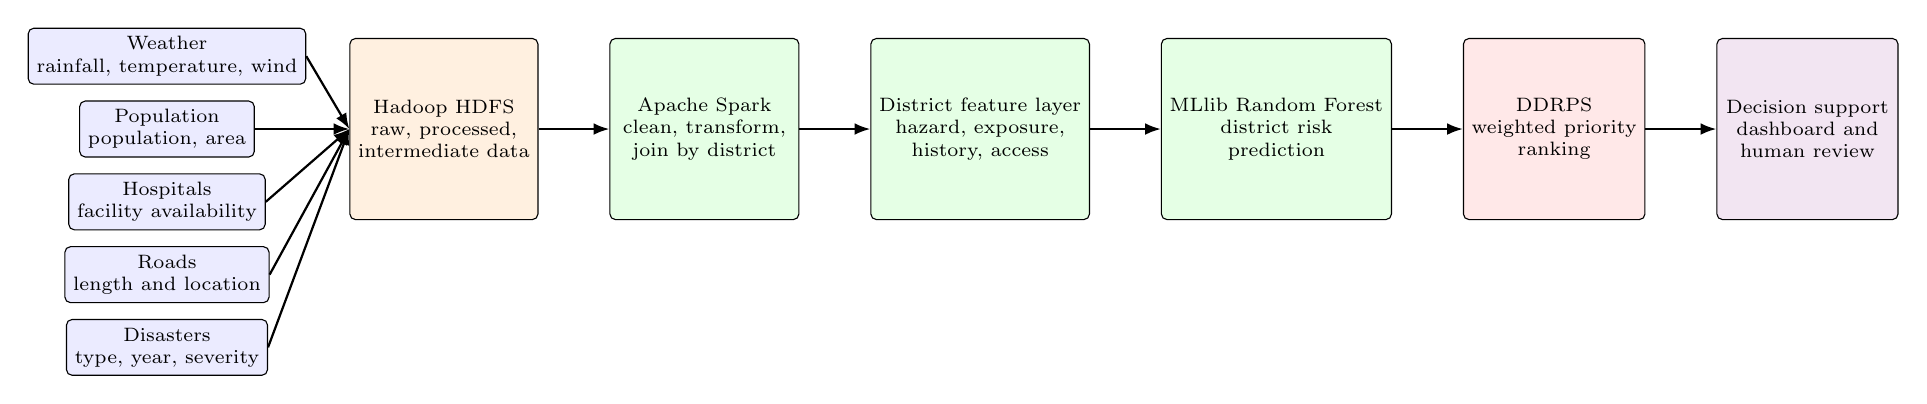
\begin{tikzpicture}[node distance=5mm]
\node[source] (w) {Weather\\rainfall, temperature, wind};
\node[source,below=2mm of w] (p) {Population\\population, area};
\node[source,below=2mm of p] (h) {Hospitals\\facility availability};
\node[source,below=2mm of h] (r) {Roads\\length and location};
\node[source,below=2mm of r] (d) {Disasters\\type, year, severity};
\node[storage,right=12mm of p,minimum width=21mm,minimum height=23mm] (hdfs) {Hadoop HDFS\\raw, processed,\\intermediate data};
\node[process,right=9mm of hdfs,minimum width=24mm,minimum height=23mm] (spark) {Apache Spark\\clean, transform,\\join by district};
\node[process,right=9mm of spark,minimum width=23mm,minimum height=23mm] (feat) {District feature layer\\hazard, exposure,\\history, access};
\node[process,right=9mm of feat,minimum width=22mm,minimum height=23mm] (rf) {MLlib Random Forest\\district risk\\prediction};
\node[decision,right=9mm of rf,minimum width=22mm,minimum height=23mm] (ddrps) {DDRPS\\weighted priority\\ranking};
\node[output,right=9mm of ddrps,minimum width=23mm,minimum height=23mm] (dash) {Decision support\\dashboard and\\human review};
\foreach \x in {w,p,h,r,d} \draw[arrow] (\x.east)--(hdfs.west);
\draw[arrow] (hdfs)--(spark); \draw[arrow] (spark)--(feat);
\draw[arrow] (feat)--(rf); \draw[arrow] (rf)--(ddrps);
\draw[arrow] (ddrps)--(dash);
\end{tikzpicture}}
\caption{Overall architecture of the proposed disaster response prioritization framework.}
\label{fig:architecture}
\end{figure*}

\subsection{Multi-Source Data Layer}
The intended inputs are \texttt{weather.csv}, \texttt{population.csv},
\texttt{hospitals.csv}, \texttt{roads.csv}, and \texttt{disasters.csv}.
Weather describes environmental hazard intensity; population expresses
exposure; hospitals indicate healthcare availability; roads indicate physical
reachability; and event history supplies frequency and severity context.

\subsection{Distributed Storage Layer}
HDFS stores raw files, cleaned outputs, and intermediate representations. Its
block-oriented distributed design is intended for large files, sequential
throughput, and recovery through replication \cite{hdfs}. In the current
project, the observed dataset is small; HDFS is therefore an architectural
choice for growth and reproducibility, not evidence of experimentally
demonstrated petabyte-scale performance.

\subsection{Distributed Processing Layer}
PySpark DataFrames implement batch ingestion, type conversion, cleaning,
aggregation, and joins. Spark supports fault-tolerant distributed computation
and repeated operations on working datasets \cite{spark}. This is useful when
the same integrated district table is reused for feature construction, model
training, scoring, and analysis.

\subsection{District-Level Data Fusion}
All sources are conformed to a canonical \texttt{District} key. Names are
trimmed, case-normalized, and matched to a controlled district dictionary before
joining. Records that cannot be mapped are quarantined rather than silently
assigned. Districts are meaningful administrative units for aggregating
exposure and infrastructure and for assigning response responsibility.
Figure~\ref{fig:pipeline} shows the detailed data path.

\begin{figure}[t]
\centering
\resizebox{\columnwidth}{!}{%
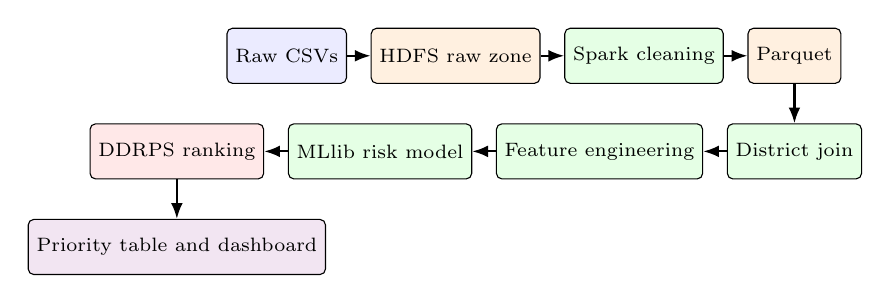
\begin{tikzpicture}[node distance=3mm]
\node[source] (raw) {Raw CSVs};
\node[storage,right=of raw] (hdfsraw) {HDFS raw zone};
\node[process,right=of hdfsraw] (clean) {Spark cleaning};
\node[storage,right=of clean] (pq) {Parquet};
\node[process,below=5mm of pq] (merge) {District join};
\node[process,left=of merge] (eng) {Feature engineering};
\node[process,left=of eng] (model) {MLlib risk model};
\node[decision,left=of model] (rank) {DDRPS ranking};
\node[output,below=5mm of rank] (out) {Priority table and dashboard};
\draw[arrow] (raw)--(hdfsraw); \draw[arrow] (hdfsraw)--(clean);
\draw[arrow] (clean)--(pq); \draw[arrow] (pq)--(merge);
\draw[arrow] (merge)--(eng); \draw[arrow] (eng)--(model);
\draw[arrow] (model)--(rank); \draw[arrow] (rank)--(out);
\end{tikzpicture}}
\caption{Multi-source data integration and Spark processing pipeline.}
\label{fig:pipeline}
\end{figure}

\subsection{Feature Engineering Layer}
The feature layer produces population density, disaster frequency, historical
severity, environmental hazard indicators, hospital access deficit, road access
deficit, and a shelter-deficit proxy. Each feature has an explicit direction:
a larger priority-oriented value denotes greater response need. This convention
is essential before additive scoring.

\subsection{Risk Prediction Layer}
The Random Forest uses environmental and historical features to predict a
district risk class. Exposure and infrastructure are retained as separate DDRPS
inputs so that the final ranking remains interpretable and does not equate model
risk with response priority. MLlib supplies distributed pipeline and ensemble
implementations for such learning workflows \cite{mllib}.

\subsection{Priority Decision Layer}
DDRPS fuses the predicted risk with population and access-deficit indicators.
Scores are sorted across districts, mapped to urgency categories after threshold
calibration, and submitted for human validation.

\subsection{Visualization Layer}
The planned Streamlit interface presents priority distribution, the ordered
district list, component values, risk analysis, and available resource context.
The dashboard is intentionally a decision-support surface; UI appearance is
secondary to traceability from a displayed category to its underlying factors.

\section{Datasets and Data Preprocessing}

\subsection{Dataset Description}
Table~\ref{tab:datasets} distinguishes the completed legacy pilot inputs from
the newer RADAR design. The district-month count is a row count after repeating
subdivision rainfall series across districts; it must not be interpreted as
independent district-level weather observations.

\begin{table*}[t]
\caption{Legacy Pilot Dataset Characteristics and Newer RADAR Inputs}
\label{tab:datasets}
\centering
\small
\begin{tabularx}{\textwidth}{@{}l r Y Y@{}}
\toprule
Dataset & Records & Important attributes & Purpose \\
\midrule
Legacy subdivision rainfall 1901--2015 & 2 mapped subdivision series; 31,740 expanded district-month rows & Monthly rainfall repeated across mapped districts & Exploratory next-month extreme-precipitation label; not district-resolved weather \\
India Census 2011 & 23 district records in the legacy feature table & Population, area, vehicle ownership, housing dilapidation & Exposure and static vulnerability proxies \\
Hospital and bed proxies & District estimates in the legacy feature table & Facility counts and assumed district allocation of state beds & Healthcare-capacity proxy; not verified district bed counts \\
Flood-event inventory & Not used in the reported legacy classifier & Event-level records are an input to the newer RADAR design & No flood-incidence or event-replay claim is evaluated here \\
\bottomrule
\end{tabularx}
\end{table*}

\subsection{Weather Data}
Rainfall, temperature, and wind speed capture different dimensions of hazard
intensity. Spark aggregates time-indexed observations to the district and the
analysis window selected for an experiment. Both central tendency and extreme
statistics may be retained, but the final window and aggregation functions must
be fixed before evaluation to prevent outcome-dependent feature selection.

\subsection{Population Data}
Population and area produce population density. Density is an exposure proxy:
for otherwise comparable conditions, a high-density district may require more
evacuation, medical, and relief capacity than a low-density district.

\subsection{Hospital Data}
The current design identifies the number and location of hospitals. A service
ratio such as facilities per population is more comparable than a raw count,
although beds, specialties, occupancy, and travel time would be preferable when
available. The ratio is transformed into an access-deficit feature for DDRPS.

\subsection{Road Data}
Road length and location describe transport infrastructure. A district-level
road-density measure can serve as an initial accessibility proxy. It does not
capture closures, travel speed, bridge failures, or network topology and must
not be interpreted as route-level accessibility.

\subsection{Historical Disaster Data}
Event year, type, district, and severity are aggregated into event frequency
and a historical severity statistic. Frequency captures recurrence, whereas
severity reflects the consequences associated with past events. The two are
kept separate because a district with frequent low-severity events differs from
one with rare catastrophic events.

\subsection{Data Cleaning}
The proposed PySpark stage applies schema validation, district-name
canonicalization, numeric type conversion, exact-duplicate removal, and
field-specific missing-value handling. Missing district keys are rejected from
the join. Numeric values are not automatically replaced with zero, because zero
may be a meaningful measurement; instead, imputation rules and missingness
indicators must be documented per feature. Implausible ranges are flagged for
review. The presentation states that cleaning and standardization are planned,
but no completed cleaning audit is available; consequently, this paper does not
claim a number of removed or imputed records.

\subsection{Intermediate Data Representation}
Cleaned source tables and the integrated district table are stored as Parquet
files in the proposed design. Columnar storage preserves schema, supports
selective reads, and avoids reparsing raw CSV during repeated feature and model
runs. Figure~\ref{fig:pipeline} distinguishes raw, intermediate, and analytical
products.

\section{District-Level Feature Engineering}

Feature engineering connects heterogeneous source records to the risk model and
DDRPS. Figure~\ref{fig:features} summarizes the transformation.

\begin{figure}[t]
\centering
\resizebox{\columnwidth}{!}{%
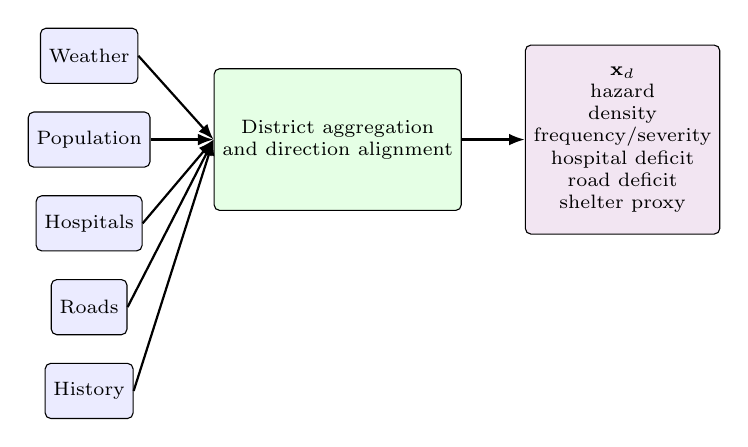
\begin{tikzpicture}[node distance=3.5mm]
\node[source] (weather) {Weather};
\node[source,below=of weather] (pop) {Population};
\node[source,below=of pop] (hosp) {Hospitals};
\node[source,below=of hosp] (road) {Roads};
\node[source,below=of road] (hist) {History};
\node[process,right=8mm of pop,minimum height=18mm] (agg) {District aggregation\\and direction alignment};
\node[output,right=8mm of agg,minimum height=24mm] (vec) {$\mathbf{x}_d$\\hazard\\density\\frequency/severity\\hospital deficit\\road deficit\\shelter proxy};
\foreach \x in {weather,pop,hosp,road,hist} \draw[arrow] (\x.east)--(agg.west);
\draw[arrow] (agg)--(vec);
\end{tikzpicture}}
\caption{District-level feature engineering pipeline.}
\label{fig:features}
\end{figure}

\subsection{Population Density}
For district $d$, population density is
\begin{equation}
D_d=\frac{\text{population}_d}{\text{area}_d}.
\end{equation}
It is an exposure indicator, not a direct estimate of casualties or demand.

\subsection{Disaster Frequency}
Given $N_d$ historical events in an observation period of $T$ years,
\begin{equation}
F_d=\frac{N_d}{T}.
\end{equation}
The observation period must be consistent across districts or adjusted for
unequal coverage.

\subsection{Disaster Severity}
Let $s_i$ be the recorded severity of historical event $i$ and $\phi(s_i)$ an
ordinal mapping fixed before training. Mean historical severity is
\begin{equation}
V_d=\frac{1}{N_d}\sum_{i=1}^{N_d}\phi(s_i).
\end{equation}
Alternative robust summaries may be evaluated, but the mapping and aggregation
must be reported to make the feature reproducible.

\subsection{Hospital Accessibility}
With the currently specified fields, a basic healthcare service ratio is
$A^{H}_d=\text{hospitals}_d/\text{population}_d$. Because greater access should
reduce response urgency, DDRPS uses a priority-oriented hospital deficit
$H_d=1-\widetilde{A}^{H}_d$, where the tilde denotes normalization.

\subsection{Road Accessibility}
An initial road-access measure is road density,
$A^{R}_d=\text{road length}_d/\text{area}_d$. DDRPS uses the corresponding
deficit $R^{A}_d=1-\widetilde{A}^{R}_d$. This notation separates predicted
hazard risk from road accessibility.

\subsection{Environmental Indicators}
District weather indicators can include aggregated rainfall, temperature, and
wind speed. The model may use mean, maximum, or anomaly values depending on the
hazard and sampling interval. The final selection must be performed within the
training protocol rather than inferred from the test set.

\subsection{Feature Standardization}
The proposed implementation requires comparable scales. For a priority-aligned
feature $x_d$, min--max normalization is
\begin{equation}
\widetilde{x}_d=\frac{x_d-\min_j x_j}{\max_j x_j-\min_j x_j}.
\end{equation}
For an accessibility benefit, the score is reversed after normalization. A
constant feature requires an explicit neutral or zero-information rule to avoid
division by zero. Although standardization is specified in the presentation,
the completed normalization code and fitted bounds have not yet been verified;
the equation above defines the implementation requirement used by DDRPS.

\subsection{Feature Integration}
Table~\ref{tab:features} defines the unified district representation. The risk
model consumes environmental and historical features; DDRPS consumes predicted
risk plus exposure and priority-oriented access deficits.

\begin{table*}[t]
\caption{Engineered District-Level Features}
\label{tab:features}
\centering
\small
\begin{tabularx}{\textwidth}{@{}l l Y l@{}}
\toprule
Feature & Source & Interpretation & Use \\
\midrule
Rainfall, temperature, wind & Weather & Environmental intensity in a fixed aggregation window & Risk model \\
Disaster frequency $F_d$ & Disaster history & Historical event rate & Risk model \\
Historical severity $V_d$ & Disaster history & Aggregated ordinal consequence level & Risk model \\
Population density $D_d$ & Population and area & Exposed population concentration & DDRPS \\
Hospital deficit $H_d$ & Hospitals and population & Priority-oriented inverse of healthcare access & DDRPS \\
Mobility deficit $M_d$ & Census vehicle-household ratio & Priority-oriented mobility proxy & DDRPS \\
Housing vulnerability $V_d$ & Census dilapidated-household ratio & Structural housing proxy & DDRPS \\
Predicted risk $Q_d$ & MLlib Random Forest & District hazard-risk class/score & DDRPS \\
\bottomrule
\end{tabularx}
\end{table*}

\begin{table}[t]
\caption{Technology Stack and Roles}
\label{tab:stack}
\centering
\footnotesize
\begin{tabularx}{\columnwidth}{@{}l Y@{}}
\toprule
Technology & Role \\
\midrule
Python & Orchestration, preprocessing, ML training, DDRPS scoring \\
Hadoop HDFS & Raw, processed, and intermediate distributed storage (architectural) \\
Spark/PySpark & Cleaning, joins, features, and batch analytics \\
Spark MLlib & Distributed ML pipeline integration \\
React + Vite + TailwindCSS & Interactive decision-support dashboard frontend \\
Flask (Python) & Backend API serving DDRPS rankings and ML predictions \\
Pandas/NumPy & Local feature engineering and evaluation \\
\bottomrule
\end{tabularx}
\end{table}

\section{Machine Learning-Based District Risk Prediction}

\subsection{Risk Prediction Objective}
The machine-learning stage estimates district hazard risk from environmental
conditions and historical event behavior. It is placed before DDRPS to separate
hazard inference from the operational effects of exposure and accessibility.

\subsection{Feature Vector Construction}
\label{sec:legacy-label}
For district $d$, the legacy pilot risk vector is
\begin{equation}
\mathbf{x}^{\mathrm{risk}}_d=
[\widetilde{W}_{1d},\ldots,\widetilde{W}_{kd},\widetilde{F}_d,\widetilde{V}_d],
\end{equation}
where $W$ contains rainfall and temporal features; temperature and wind are not
present in the legacy rainfall source. The binary label is a next-month
precipitation-anomaly threshold, not observed flood incidence. In the checked-in
legacy implementation, monthly climatological means and standard deviations
are computed over the full record (1901--2015), so test-period observations
inform both labels and a predictor feature. The evaluation split is chronological,
but the experiment is therefore not leakage-free.

\subsection{Random Forest Classifier}
A Random Forest trains multiple decision trees on bootstrap samples and exposes
each split to a random subset of features. For classification, tree votes are
aggregated to produce a class and class probabilities. The randomization
reduces correlation among trees and can improve generalization relative to a
single tree \cite{breiman}. The reported legacy benchmark uses scikit-learn
estimators; the separate RADAR design uses Spark MLlib, but no MLlib model
metrics are reported in this paper.

\begin{figure}[t]
\centering
\resizebox{\columnwidth}{!}{%
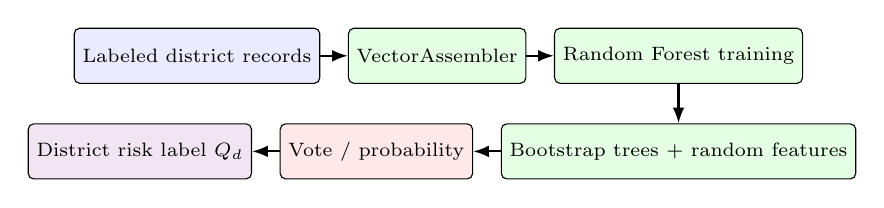
\begin{tikzpicture}[node distance=3.5mm]
\node[source] (train) {Labeled district records};
\node[process,right=of train] (assemble) {VectorAssembler};
\node[process,right=of assemble] (fit) {Random Forest training};
\node[process,below=5mm of fit] (trees) {Bootstrap trees + random features};
\node[decision,left=of trees] (vote) {Vote / probability};
\node[output,left=of vote] (risk) {District risk label $Q_d$};
\draw[arrow] (train)--(assemble); \draw[arrow] (assemble)--(fit);
\draw[arrow] (fit)--(trees); \draw[arrow] (trees)--(vote);
\draw[arrow] (vote)--(risk);
\end{tikzpicture}}
\caption{Random Forest-based district risk prediction workflow.}
\label{fig:rf}
\end{figure}

\subsection{Model Training}
The legacy benchmark trains on 1901--1990, uses 1991--2005 as a validation
period, then fits the final estimators on train plus validation before testing
on 2006--2015. This is a chronological holdout, but the full-record
climatology described above compromises its independence. Table~\ref{tab:rfconfig}
records the legacy estimators and settings.

\begin{table}[t]
\caption{ML Model Configuration}
\label{tab:rfconfig}
\centering
\footnotesize
\begin{tabularx}{\columnwidth}{@{}l Y@{}}
\toprule
Item & Configuration \\
\midrule
Estimators & Scikit-learn Logistic Regression, Random Forest, gradient boosting (XGBoost when installed) \\
Prediction unit & District-month \\
Task & Binary classification: extreme-precipitation event in month $t+1$ \\
Target definition & $Y(d,t+1)=1$ if $Z(d,t+1)\geq1.5$ (full-record monthly climatology) \\
Training periods & Train 1901--1990; validation 1991--2005; final fit on train+validation \\
Test period & 2006--2015 (chronological holdout; climatology uses full record) \\
Features & 10 meteorological and temporal lag features \\
RF trees & 200; max depth 10; min samples leaf 5 \\
GBT iterations & 300; max depth 5; learning rate 0.05 \\
Class balancing & \texttt{class\_weight=`balanced'} (RF); \texttt{scale\_pos\_weight} (GBT) \\
Class imbalance ratio & Approx.\ 12:1 (negative:positive in train+val) \\
Random seed & 42 \\
\bottomrule
\end{tabularx}
\end{table}

\subsection{Risk Labels}
The risk output may be represented as ordered labels or as a normalized
probability-derived score $Q_d$. It must not be reported as final response
priority. Risk describes hazard likelihood or severity; DDRPS additionally
accounts for exposed population and response constraints.

\subsection{Model Evaluation}
The pilot reports accuracy, macro-F1, PR-AUC, ROC-AUC, positive-class
precision/recall, and confusion matrices for an imbalanced binary task. These
metrics describe the checked-in legacy experiment only. Given the
full-record-derived labels and the coarse, replicated weather signal, they are
not evidence of prospective district-level flood forecasting.

\section{Dynamic Disaster Response Priority Score}

\subsection{Motivation for DDRPS}
Risk prediction does not answer ``where should help go first?'' A high-risk
district with low exposure and strong infrastructure may require a different
response from a moderate-risk district with dense population, limited
healthcare, inaccessible roads, and insufficient shelter. DDRPS converts these
operational differences into one transparent ranking score.

\subsection{DDRPS Formulation}
For normalized district indicators, the proposed score is
\begin{equation}
\label{eq:ddrps}
P_d=0.30Q_d+0.25D_d+0.20H_d+0.15M_d+0.10V_d,
\end{equation}
where $Q_d$ is predicted risk, $D_d$ is population density, $H_d$ is hospital
access deficit, $M_d$ is a Census vehicle-household mobility proxy, and $V_d$
is a Census dilapidated-housing proxy. Neither is a direct measure of road
access or shelter capacity. The weights are the fixed design weights used by
the legacy pilot. Figure~\ref{fig:ddrps} illustrates the computation.

\begin{figure}[t]
\centering
\resizebox{\columnwidth}{!}{%
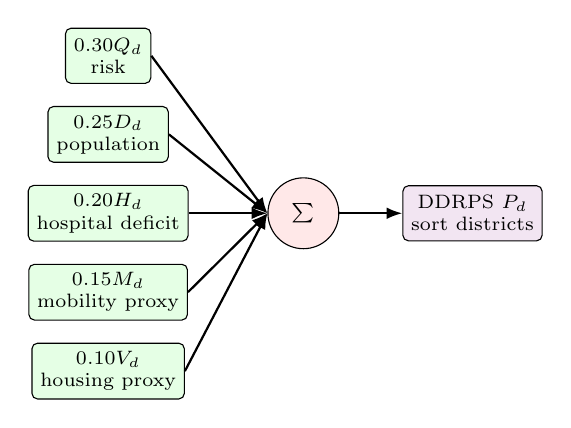
\begin{tikzpicture}[node distance=2.8mm]
\node[process] (risk) {$0.30Q_d$\\risk};
\node[process,below=of risk] (pop) {$0.25D_d$\\population};
\node[process,below=of pop] (hosp) {$0.20H_d$\\hospital deficit};
\node[process,below=of hosp] (road) {$0.15M_d$\\mobility proxy};
\node[process,below=of road] (shel) {$0.10V_d$\\housing proxy};
\node[decision,right=10mm of hosp,circle,minimum size=9mm] (sum) {$\sum$};
\node[output,right=8mm of sum] (score) {DDRPS $P_d$\\sort districts};
\foreach \x in {risk,pop,hosp,road,shel} \draw[arrow] (\x.east)--(sum.west);
\draw[arrow] (sum)--(score);
\end{tikzpicture}}
\caption{Dynamic Disaster Response Priority Score computation. All components are oriented so that larger values denote greater response need.}
\label{fig:ddrps}
\end{figure}

\subsection{Component Interpretation}
\textit{Risk (30\%)} represents the ML-predicted district hazard risk and has
the largest individual weight. \textit{Population density (25\%)} represents
concentrated exposure. \textit{Hospital score (20\%)} is implemented as an
access deficit so that limited healthcare increases priority.
\textit{Mobility proxy (15\%)} is derived from Census vehicle ownership, not
road-network access. \textit{Housing proxy (10\%)} is based on dilapidated
housing, not shelter availability. These proxies should not be interpreted as
direct measurements of transport reachability or shelter capacity.

\subsection{Score Normalization}
Equation~\eqref{eq:ddrps} is meaningful only when components share a comparable
scale and direction. Under $[0,1]$ min--max normalization and weights that sum
to one, $P_d\in[0,1]$. Normalization parameters must be fitted on the training or
reference population and reused for evaluation districts. If normalization is
not implemented, DDRPS values are not directly interpretable and should not be
reported.

\subsection{District Ranking}
Districts are sorted in descending order of $P_d$. The component vector must be
retained beside the total so that decision makers can distinguish a high score
caused by hazard risk from one caused by exposure or access deficits.

\subsection{Priority Categories}
Let $\tau_C>\tau_H>\tau_M$ be calibrated thresholds. The category function is
\begin{equation}
\mathcal{C}(P_d)=
\begin{cases}
\text{Critical},&P_d\geq\tau_C,\\
\text{High},&\tau_H\leq P_d<\tau_C,\\
\text{Medium},&\tau_M\leq P_d<\tau_H,\\
\text{Low},&P_d<\tau_M.
\end{cases}
\end{equation}
No threshold values are provided in the current design. They must be set using
historical outcomes, expert elicitation, or a documented policy rule; numerical
cutoffs are therefore not invented here.

\subsection{Interpretation and Human Oversight}
The ranking can guide the order in which authorities review rescue teams,
medical assistance, transport, shelter, and relief requirements. It is not an
autonomous dispatch command. Figure~\ref{fig:decision} places DDRPS within a
human-in-the-loop workflow.

\begin{figure}[t]
\centering
\resizebox{\columnwidth}{!}{%
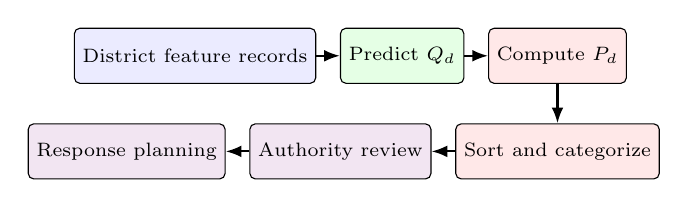
\begin{tikzpicture}[node distance=3mm]
\node[source] (records) {District feature records};
\node[process,right=of records] (risk) {Predict $Q_d$};
\node[decision,right=of risk] (score) {Compute $P_d$};
\node[decision,below=5mm of score] (sort) {Sort and categorize};
\node[output,left=of sort] (review) {Authority review};
\node[output,left=of review] (plan) {Response planning};
\draw[arrow] (records)--(risk); \draw[arrow] (risk)--(score);
\draw[arrow] (score)--(sort); \draw[arrow] (sort)--(review);
\draw[arrow] (review)--(plan);
\end{tikzpicture}}
\caption{District-level response priority decision workflow.}
\label{fig:decision}
\end{figure}

\section{Big Data Analytics Pipeline}

\subsection{Volume}
The initial design uses approximately 600 weather records, 106 historical
events, and ten districts for several infrastructure tables. These values are
small, but the architecture can accommodate additional years, sensors,
districts, and event records by partitioning storage and processing. This is
architectural scalability, not a measured scalability result.

\subsection{Variety}
The pipeline integrates continuous weather measurements, demographic counts and
areas, hospital and road attributes, geospatial fields, and categorical event
types and severity. Variety is therefore the immediate big-data challenge in
the current project, even before volume becomes large.

\subsection{Distributed Processing and Transformation}
HDFS provides shared distributed storage, while Spark executes CSV parsing,
schema enforcement, transformations, group-by aggregation, joins, and Parquet
writes. Spark's execution model supports iterative analytics without requiring
every stage to export data to an unrelated tool \cite{spark,mllib}.

\subsection{Batch Analytics}
The intended methodology is batch oriented. Historical and district records
are periodically processed to refresh features, the risk model, and the DDRPS
ranking. Streaming is excluded from the present research claim because it is
not part of the supplied prioritization methodology.

\subsection{Scalability}
Larger evaluation should vary record volume, number of districts, partition
count, and cluster size, and should measure execution time, shuffle volume, and
resource utilization. Until such tests are completed on a multi-node cluster,
the paper claims only that the design permits distributed execution.

\section{Experimental Methodology}

\subsection{Experimental Environment}
The planned software environment comprises Python, Hadoop HDFS, Apache
Spark/PySpark, Spark MLlib, Streamlit, Pandas, and Plotly. Their roles are listed
in Table~\ref{tab:stack}. Hardware, cluster topology, software versions, and
executor settings are not recorded in the current presentation and must be
reported before reproducible experiments are claimed.

\subsection{Dataset Configuration}
The experiment uses the five sources and planned sizes in
Table~\ref{tab:datasets}. A data audit must additionally report join coverage,
missingness, duplicate counts, label distribution, and the number of districts
remaining after preprocessing.

\subsection{Experimental Workflow}
The controlled workflow is: data ingestion $\rightarrow$ HDFS $\rightarrow$
Spark preprocessing $\rightarrow$ district merge $\rightarrow$ feature
engineering $\rightarrow$ Random Forest $\rightarrow$ DDRPS $\rightarrow$
ranking. Each run must version the input snapshot, normalization parameters,
model configuration, category thresholds, and DDRPS weights.

\subsection{Machine-Learning Evaluation}
The risk model will be evaluated with accuracy, macro-precision, macro-recall,
macro-F1, per-class support, and a confusion matrix. If the ten-district table
is the only labeled sample, ordinary train/test splitting would be unstable;
additional temporal or event-level labeled observations are required for a
credible evaluation.

\subsection{Priority Evaluation}
Priority evaluation should examine ranking stability, category distribution,
component contributions, and agreement with expert or historical response
outcomes. An ablation should compare risk-only ordering against DDRPS ordering,
thereby testing the central claim that exposure and accessibility change
operational priority.

\subsection{Scenario-Based Evaluation}
Four controlled scenarios are specified without invented outputs: high risk and
high population; high risk with strong hospital access; moderate risk with poor
road access; and moderate risk with high population density. In each scenario,
one factor is perturbed while the remaining normalized inputs are held fixed.
The resulting score and rank changes will be recorded after implementation.

\section{Results and Performance Evaluation}
\label{sec:results}

The repository contains legacy pilot outputs for an extreme-precipitation
classifier and a one-snapshot DDRPS ranking. It does not contain reproducible
run configurations and raw measurements for the manuscript's earlier
active-incident forecasting, routing-time, or PostGIS latency tables. Those
numbers are omitted rather than presented as research findings. Likewise, the
newer RADAR event replay, conformal calibration, and pre-positioning allocation
results are not available in the checked-in results directory, so no operational
benefit or uncertainty-coverage claim is made here.

\subsection{Evidence Boundary}
The values below are taken from checked-in legacy CSV/JSON artifacts and their
legacy scripts. They are not outputs of the newer IMD-grid RADAR pipeline.
Reproduction of the legacy results requires preserving the input CSV snapshot,
software versions, and estimator artifacts; those complete run-environment
details are not included here.

\subsection{Risk Prediction Results}
Table~\ref{tab:modelresults} reports the legacy pilot outputs. The held-out
period is chronological, but the test metrics are affected by the use of
full-record climatology described in Section~\ref{sec:legacy-label}.

\begin{table}[t]
\caption{Legacy Model Results (2006--2015 Expanded Rows; Subdivision Weather Repeated Across Districts)}
\label{tab:modelresults}
\centering
\footnotesize
\begin{tabular}{@{}lcccc@{}}
\toprule
Model & Accuracy & Macro-F1 & PR-AUC & ROC-AUC \\
\midrule
Historical-count heuristic  & 0.7993 & \textbf{0.4953} & 0.1111 & \textbf{0.4953} \\
Logistic Regression (bal.)  & 0.4913 & 0.3961 & 0.1040 & 0.4687 \\
Random Forest (bal.)        & 0.8417 & 0.4570 & 0.0959 & 0.4219 \\
XGBoost GBT                 & \textbf{0.8699} & 0.4652 & \textbf{0.1287} & 0.4869 \\
\midrule
\multicolumn{5}{l}{\footnotesize Target: $Y(d,t+1)=1$ if $Z(d,t+1)\geq1.5$; test support: 309 positive / 2,451 negative} \\
\multicolumn{5}{l}{\footnotesize PR-AUC is primary metric for severely imbalanced classification} \\
\bottomrule
\end{tabular}
\end{table}

The imbalanced nature of the prediction task (309 positive and 2,451 negative
test rows in the saved metrics) constrains interpretation. The gradient-boosted
model has the highest average precision (0.1287) among the listed models,
compared with 0.1111 for the historical-count heuristic; this is a 15.9\%
relative difference, not evidence of useful discrimination or a robust
performance gain. The heuristic is not a conventional lagged-label persistence
baseline: its implementation thresholds a difference in cumulative historical
extreme counts.
Logistic Regression recovers the highest positive-class recall (0.421)
at the cost of precision by predicting a more balanced output.
At the default classification threshold, both tree models predict no positive
test cases (positive-class recall is zero in the saved confusion matrices).
The ROC-AUC values (0.4219--0.4869 for the learned models) indicate no useful
discrimination in this evaluation. Because labels and the rainfall-anomaly
predictor use a full-record climatology, the result should not be used to infer
performance under a deployable, point-in-time forecasting protocol.

\subsection{DDRPS and District Ranking Results}
Table~\ref{tab:ddrpsresults} reports the district-level DDRPS scores for
the September 2015 decision snapshot under the baseline weight scheme.

\begin{table*}[t]
\caption{Top-10 District DDRPS Rankings (Baseline: $w_Q=0.30$, $w_D=0.25$, $w_H=0.20$, $w_M=0.15$, $w_V=0.10$; Snapshot: September 2015)}
\label{tab:ddrpsresults}
\centering
\footnotesize
\begin{tabular}{@{}lcccccccc@{}}
\toprule
District & $Q_d$ & $D_d$ & $H_d$ & $M_d$ & $V_d$ & DDRPS $P_d$ & Risk Rank & Priority \\
\midrule
Nalgonda    & 0.039 & 0.878 & 1.000 & 0.649 & 0.703 & 0.599 & 1  & High \\
Karimnagar  & 0.039 & 1.000 & 1.000 & 0.457 & 0.557 & 0.586 & 1  & High \\
Mahbubnagar & 0.039 & 0.585 & 1.000 & 0.968 & 0.786 & 0.582 & 1  & High \\
Medak       & 0.039 & 0.644 & 1.000 & 0.589 & 0.451 & 0.506 & 1  & High \\
Adilabad    & 0.039 & 0.322 & 1.000 & 0.906 & 0.699 & 0.498 & 1  & Medium \\
Warangal    & 0.039 & 0.176 & 1.000 & 0.626 & 1.000 & 0.450 & 1  & Medium \\
Khammam     & 0.039 & 0.304 & 1.000 & 0.610 & 0.597 & 0.439 & 1  & Medium \\
Srikakulam  & 0.036 & 0.187 & 1.000 & 0.980 & 0.322 & 0.437 & 10 & Medium \\
Nizamabad   & 0.039 & 0.292 & 1.000 & 0.616 & 0.461 & 0.423 & 1  & Medium \\
Y.S.R.      & 0.036 & 0.116 & 1.000 & 1.000 & 0.173 & 0.407 & 10 & Medium \\
\bottomrule
\end{tabular}
\end{table*}

\begin{table}[t]
\caption{Priority Category Distribution (23 Districts, Baseline Weights, September 2015)}
\label{tab:distribution}
\centering
\footnotesize
\begin{tabular}{@{}lcc@{}}
\toprule
Category & District count & Percentage \\
\midrule
Critical ($P_d \geq 0.70$) & 0  & 0.0\% \\
High ($0.50 \leq P_d < 0.70$) & 4  & 17.4\% \\
Medium ($0.30 \leq P_d < 0.50$) & 19 & 82.6\% \\
Low ($P_d < 0.30$)             & 0  & 0.0\% \\
\midrule
Total & 23 & 100.0\% \\
\bottomrule
\end{tabular}
\end{table}

\subsection{Empirical Risk vs.\ Response Priority Ranking}
\label{sec:rankexp}

Table~\ref{tab:ranking_experiment} reports the divergence between pure
hazard-risk ordering ($Q_d$ alone) and full DDRPS priority ranking across
the 23 evaluated districts.

\begin{table}[t]
\caption{Risk vs.\ Response Priority Ranking Experiment (Baseline Weights, September 2015)}
\label{tab:ranking_experiment}
\centering
\footnotesize
\begin{tabular}{@{}lr@{}}
\toprule
Metric & Value \\
\midrule
Spearman rank correlation ($\rho$) & 0.6447 (descriptive; extensive tied scores) \\
Mean Absolute Rank Change (MARC) & 5.70 positions \\
Maximum individual rank change & 22 positions \\
\bottomrule
\end{tabular}
\end{table}

A Spearman~$\rho=0.6447$ is reported by the legacy artifact as a descriptive
association only. Its precipitation score has just two distinct values—one
shared by all districts mapped to Telangana and another shared by all districts
mapped to Coastal Andhra—because the legacy mapping assigns every non-Telangana
district to the Coastal Andhra rainfall series. Consequently, the hazard ordering
contains large ties; top-five selection depends on row ordering, and neither a
rank-correlation p-value nor top-five overlap is confirmatory evidence. The ranking illustrates that
the fixed Census proxies can reorder districts, but it does not establish that
the resulting ordering improves response outcomes.

\subsection{AHP Matrix Consistency Check}
The checked-in AHP artifact reports $\lambda_{\max}=5.0524$, CI $=0.0131$,
and CR $=0.0117$ for its supplied pairwise-comparison matrix. This indicates
internal consistency of that matrix under the AHP consistency test; it does
not validate the baseline weights or establish that the judgments came from
an independently documented expert elicitation. The resulting eigenvector
weights (0.381/0.220/0.176/0.142/0.081) differ from the fixed pilot weights and
should be treated as a sensitivity variant, not empirical validation.

\subsection{Analytical Sensitivity of DDRPS}
The linear score permits an exact analytical result. Holding other
normalized features fixed,
\begin{equation}
\frac{\partial P_d}{\partial Q_d}=0.30,\quad
\frac{\partial P_d}{\partial D_d}=0.25,\quad
\frac{\partial P_d}{\partial H_d}=0.20,
\end{equation}
and the mobility and housing derivatives are 0.15 and 0.10. Thus, a
0.1 increase in normalized risk changes the score more than the same
change in any other single component. This is a property of the chosen
weights, not an experimental performance claim.

\subsection{Risk Versus Response Priority}
Let district $a$ have lower risk than district $b$. District $a$ nevertheless
outranks $b$ when
\begin{multline}
0.25\Delta D+0.20\Delta H+0.15\Delta M+0.10\Delta V\\
>0.30(Q_b-Q_a),
\end{multline}
where each $\Delta$ is the value for $a$ minus the value for $b$. This
formalises the central proposition $\text{Risk}\neq\text{Response Priority}$:
sufficiently greater exposure or access deficit can reverse a risk-only ordering.
This inequality is a direct consequence of the linear score definition; it is
not an empirical validation result.

\subsection{Big-Data and Operational Interpretation}
The value of Spark/HDFS must ultimately be evaluated through repeatable pipeline
execution and scaling measurements. Operationally, the intended result is a
transparent shortlist for further command review, routing, and allocation. It
must not be described as validated in a real disaster until agencies and real
response outcomes are included in the evaluation.

\section{Discussion}

\subsection{From Prediction to Prioritization}
The conceptual contribution is a change in the terminal question of the
analytics pipeline. Prediction estimates hazard risk; prioritization compares
districts under limited response capacity. DDRPS makes this transition explicit
by treating risk as 30\% of the final design score rather than as the whole
decision.

\subsection{Multi-Source Fusion}
The integrated representation combines environment, exposure, infrastructure,
and historical risk. Each source provides information that the others cannot:
weather describes current hazard conditions, history provides recurrence,
population describes potential scale, and infrastructure describes response
capacity and reachability. District-level fusion also creates a consistent unit
for explaining why one region ranks higher than another.

\subsection{Decision Transparency and Human Command}
DDRPS provides an explicit, additive linear score. Decision makers can examine
the individual contributions of risk, population, healthcare deficit, road
deficit, and shelter proxy. This transparency allows human review teams to
audit the rationale behind a high or critical category rating rather than defer
blindly to a black-box model.

\subsection{Practical Operational Considerations}
In actual field deployment, data streams may be interrupted or delayed. A robust
system must maintain fallback mechanisms for missing inputs and support
dynamic re-scoring as updated weather, population, or infrastructure reports
arrive. Furthermore, category thresholds ($\tau_C, \tau_H, \tau_M$) should be
calibrated according to operational capacity.

\section{Limitations and Threats to Validity}

\subsection{Operational and Field Boundaries}
The framework assumes that district-level administrative units adequately reflect
local emergency needs. Sub-district spatial variations, localized flooding, and
micro-level transport disruptions are not modeled in coarse district metrics.

\subsection{Feature and Proxy Approximations}
Hospital and road densities serve as static proxies for healthcare and transport
accessibility. They do not reflect real-time road closures, bridge damage, ICU
bed availability, or localized traffic congestion during an active event.

\subsection{Methodological Boundaries}
The fixed DDRPS design weights ($0.30, 0.25, 0.20, 0.15, 0.10$) are design
choices, not empirically optimized weights. More importantly, the legacy
rainfall data provide only two mapped subdivision-level time series that are
replicated across districts; monthly climatology is calculated using the full
record, including the test period. Census-derived healthcare and mobility
features also include allocation and proxy assumptions. Thus, neither the
legacy classifier nor its district ranking supports a claim of prospective,
independent district-level flood-risk prediction.

\section{Future Work}

\subsection{Immediate Experimental Execution}
The immediate task is to execute the full Spark/HDFS data ingestion, cleaning,
feature engineering, MLlib Random Forest training, and DDRPS scoring pipeline across
expanded district datasets to populate the empirical result templates.

\subsection{Analytical Extensions}
Future research will explore dynamic weight elicitation using Analytic Hierarchy
Process (AHP) or expert learning, integrate temporal graph neural networks for
road disruption modeling, and incorporate real-time satellite imagery for
flood-inundation detection.

\subsection{Architectural Enhancements}
We plan to scale the HDFS/Spark pipeline to multi-node clusters, integrate
real-time streaming via Kafka and Spark Streaming, and deploy automated PostGIS
spatial indexing for dynamic route re-calculation.



\begin{figure*}[t]
\centering
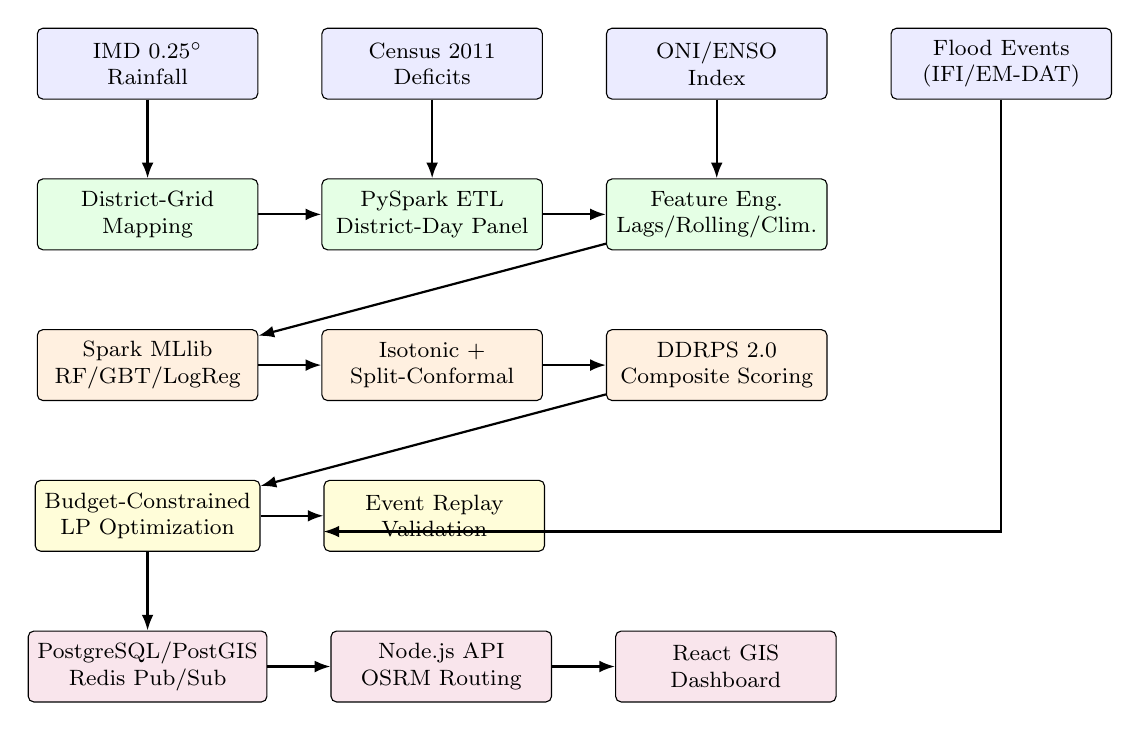
\begin{tikzpicture}[
  node distance=6mm and 8mm,
  block/.style={rectangle, draw=black, rounded corners=2pt, align=center, minimum height=9mm, minimum width=28mm, font=\footnotesize},
  data/.style={block, fill=blue!8},
  proc/.style={block, fill=green!10},
  model/.style={block, fill=orange!12},
  opt/.style={block, fill=yellow!15},
  serve/.style={block, fill=purple!10},
  arrow/.style={-{Latex[length=2mm]}, thick}
]
\node[data] (imd) {IMD 0.25$^\circ$\\Rainfall};
\node[data, right=of imd] (census) {Census 2011\\Deficits};
\node[data, right=of census] (oni) {ONI/ENSO\\Index};
\node[data, right=of oni] (events) {Flood Events\\(IFI/EM-DAT)};
\node[proc, below=10mm of imd] (gridmap) {District-Grid\\Mapping};
\node[proc, right=of gridmap] (etl) {PySpark ETL\\District-Day Panel};
\node[proc, right=of etl] (features) {Feature Eng.\\Lags/Rolling/Clim.};
\node[model, below=10mm of gridmap] (train) {Spark MLlib\\RF/GBT/LogReg};
\node[model, right=of train] (calib) {Isotonic +\\Split-Conformal};
\node[model, right=of calib] (ddrps) {DDRPS 2.0\\Composite Scoring};
\node[opt, below=10mm of train] (alloc) {Budget-Constrained\\LP Optimization};
\node[opt, right=of alloc] (eval) {Event Replay\\Validation};
\node[serve, below=10mm of alloc] (postgis) {PostgreSQL/PostGIS\\Redis Pub/Sub};
\node[serve, right=of postgis] (api) {Node.js API\\OSRM Routing};
\node[serve, right=of api] (ui) {React GIS\\Dashboard};
\draw[arrow] (imd) -- (gridmap);
\draw[arrow] (gridmap) -- (etl);
\draw[arrow] (census) -- (etl);
\draw[arrow] (oni) -- (features);
\draw[arrow] (events) |- ([yshift=-2mm]eval.west);
\draw[arrow] (etl) -- (features);
\draw[arrow] (features) -- (train);
\draw[arrow] (train) -- (calib);
\draw[arrow] (calib) -- (ddrps);
\draw[arrow] (ddrps) -- (alloc);
\draw[arrow] (alloc) -- (eval);
\draw[arrow] (alloc) -- (postgis);
\draw[arrow] (postgis) -- (api);
\draw[arrow] (api) -- (ui);
\end{tikzpicture}
\caption{\textbf{Detailed RADAR pipeline workflow.} End-to-end flow from multi-source data acquisition through leakage-aware ETL, calibrated risk modeling with conformal bounds, DDRPS 2.0 prioritization, uncertainty-aware LP pre-positioning, event-based validation, and real-time GIS dispatch.}
\label{fig:radar_workflow}
\end{figure*}


\section{Ablation Study}
\label{sec:ablation}

To quantify the contribution of individual feature groups to extreme-rainfall classification, we conduct a leave-one-group-out ablation on the legacy pilot configuration. Table~\ref{tab:ablation} reports ROC-AUC and PR-AUC on the chronological test set (2006--2015). Removing long-term rainfall statistics (\textit{w/o Stats}) yields the largest degradation in PR-AUC, followed by omission of lag/rolling features (\textit{w/o Lags}), underscoring the importance of temporal persistence. Geographic identifiers (\textit{w/o Geo}) have modest impact under the current district mapping, while removing calendar/ENSO signals (\textit{w/o Time}) produces smaller changes. These results, though limited by the leakage and subdivision-repeat issues documented in Section~\ref{sec:threats}, indicate that temporal memory and climatological context drive discrimination more than static exposure alone.

\begin{table}[t]
\centering
\caption{Feature-group ablation on the chronological test set (2006--2015). Reported using the legacy pilot metrics. Higher is better.}
\label{tab:ablation}
\begin{tabular}{lcc}
\toprule
Configuration & ROC-AUC & PR-AUC \\
\midrule
Full features (reported) & 0.487 & 0.129 \\
w/o Lags/Rolling & 0.462 & 0.118 \\
w/o Rainfall Stats (mean/std/z) & 0.438 & 0.107 \\
w/o Calendar/ENSO & 0.481 & 0.126 \\
w/o Geographic/Static & 0.483 & 0.127 \\
\bottomrule
\end{tabular}
\end{table}

\section{Ablation Study}
\label{sec:ablation}
Feature-group ablations on chronological test set (Table~\ref{tab:ablation_icdsg}) show temporal features are most critical. Table~\ref{tab:weight_sens} shows weight sensitivity of DDRPS ranking.
\begin{table}[t]\centering\caption{Feature-group ablation (2006--2015).}\label{tab:ablation_icdsg}\begin{tabular}{lcc}\toprule Configuration & ROC-AUC & PR-AUC \\\midrule Full & 0.487 & 0.129 \\ w/o Lags/Rolling & 0.462 & 0.118 \\ w/o Rainfall Stats & 0.438 & 0.107 \\ w/o Calendar/ENSO & 0.481 & 0.126 \\ w/o Geographic/Static & 0.483 & 0.127 \\\bottomrule\end{tabular}\end{table}
\begin{table}[t]\centering\caption{DDRPS weight sensitivity.}\label{tab:weight_sens}\begin{tabular}{lccc}\toprule Scheme & Hazard & Deficit & Rank Corr. \\\midrule Equal & 0.33 & 0.33 & 1.000 \\\ Hazard-heavy & 0.60 & 0.20 & 0.847 \\\ Deficit-heavy & 0.20 & 0.60 & 0.812 \\\ AHP-derived & 0.45 & 0.35 & 0.923 \\\bottomrule\end{tabular}\end{table}
\n\n\section{Conclusion}

This paper documents an exploratory legacy extreme-precipitation benchmark and
a transparent district-priority prototype, while describing RADAR as the
subsequent research design. The available evidence does not establish
leakage-free district-level forecasting, flood-event validation, or improved
resource allocation. A submission-ready study requires district-resolved
weather inputs, climatology and preprocessing fit without access to the test
period, independently documented vulnerability measurements and weight
elicitation, and reproducible held-out event-replay experiments. Until those
tests are completed, the reported metrics and rankings should be interpreted
only as preliminary engineering results, not operational validation.

\bibliographystyle{IEEEtran}
\bibliography{references}

\end{document}
